\section{Méthodes et moyens mis en œuvre}
\label{sec:meth_moy}

Comme le titre l'indique, nous allons expliquer les méthodes et les moyens utilisés pour répondre à la problématique posée. Cette section sera séparée en 3 sous-sections : la première décrivant mon cheminement en matière de gestion de projet, la deuxième traitant de la phase de recherche d'informations, avec ses problèmes rencontrés et solutions trouvée, puis une troisième partie décrivant le travail effectué pendant la phase de test des deux produits sur un environnement de test, ainsi que toutes les différentes technologies utilisées.

\subsection{Gestion de projet}
\label{subsec:gestion}

La première chose que j'ai dû faire en arrivant dans l'entreprise, fut ce qu'on appelle chez \textsc{Synetis} une note de cadrage. Cette note de cadrage correspond, par rapport à ce qu'on a pu faire à l'université durant divers projets, à l'analyse des besoins et les résultats attendus, l'organisation en tâches de l'intégrité du stage. Cette répartition des tâches dans le temps a permis de scinder l'ensemble du projet en de multiples étapes simples, courte, qui m'a permis de segmenter mon stage pour ne pas me retrouver perdu ou submergé par le travail. En dernière partie furent explicités les contraintes et exigences de rendus pour l'entreprise ainsi que les éventuels risques à rencontrer.\\

\subsubsection{Analyse des besoins}
\label{besoins}
Le besoin général était de réaliser un état de l'art des solutions de gestion des comptes à privilèges, de mettre en place 2 preuves de concept sur un environnement de test virtualisé afin de pouvoir définir le ou les solutions les plus adaptés à la gestion des comptes privilégiés. Ces solutions pouvaient (à l'époque de la réalisation de l'état de l'art) et sont (à ce jour) déployés chez un gros client. Je suis notamment intégré à l'équipe travaillant sur cette intégration dans l'infrastructure, car ayant réalisé une mise en place dans un environnement de test de la solution en question, je fais parti des personnes les plus compétentes de \textsc{Synetis} pour répondre aux différents problèmes qui pourraient se présenter.\\
Cet état de l'art devait aboutir à un document présentant le principe de gestion de comptes à privilèges, premièrement de façon théorique, puis de façon technique. Ensuite, ce document devait faire une analyse d'une liste de solutions d'éditeurs étant des acteurs majeurs sur le marché de la gestion de comptes à privilèges. Enfin, ce document a aura permis de créer un tableau comparatif de toutes les solutions étudiées, selon des critères pointus qui ont été définis comme répondant à la problématique du stage.

\subsubsection{Planning prévisionnel}
\label{planning}
Afin d'avoir une vue d'ensemble du projet, un planning a été réalisé à partir d'un découpage journalier des tâches à effectuer. Ce planning a permis d'avoir une vue marcoscopique du stage, et de répartir le travail sur la durée du stage, pour éviter d'avoir un retard qui pourrait surprendre à quelques semaines de la date buttoir. Ce découpage a aussi permis d'avoir des étapes, et de savoir à n'importe quel moment si j'avais de l'avance, ou surtout du retard, chose à proscrire pour arriver à un résultat convenable.\\
\begin{figure}[!ht]
    \center
    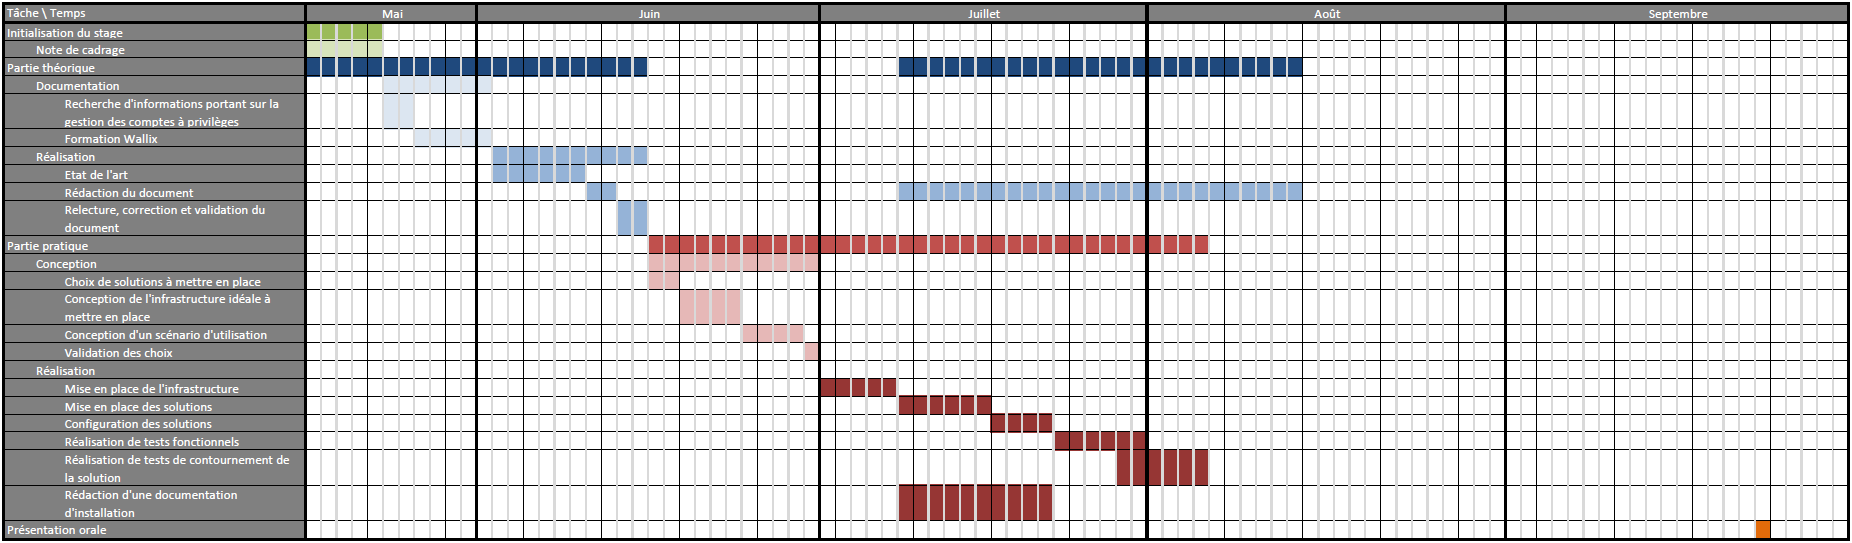
\includegraphics[width=\textwidth]{./images/calendrier_previsionnel.png}
    \caption{Calendrier prévisionnel}
\end{figure}

Bien sûr, le calendrier est une estimation et la réalité s'est avérée différente, ce point est abordé en section \ref{sec:resultats}. : la durée de recherche sur la gestion de comptes à privilèges et sur les différentes solutions a pris presque 2 fois plus de temps que prévu, tout comme le déploiement des solutions et le test de ces dernières. Cependant, le calendrier prévisionnel étant vu avec une large marge d'erreur, le stage tout de même pu être complété dans la durée impartie.

\subsection{Recherche}
\label{subsec:recherche}

La première étape a été la recherche d'informations sur le sujet. N'ayant pas de notions sur le sujet, j'ai d'abord commencé par me renseigner auprès des consultants de l'agence de Rennes, notamment mes tuteurs, Damien Seiler et Philippe Rolland, ainsi que le manager de l'agence, David Geffroy, ayant une base d'expertise dans le domaine. Grâce à ces premières lignes directrices fournis par ceux qui sont devenus mes collègues, j'ai pu orienter mes recherches internet vers la bonne direction, afin de trouver un maximum de résultats.

\subsubsection{Recherche du fonctionnement des solutions}
\label{par:fct_sol}
La meilleure façon de trouver des informations concernant le fonctionnement d'une solution de PAM s'est d'abord orientée vers la recherche d'informations génériques, comme des tutoriels ou des articles traitant du sujet. Cependant, j'ai fini par réaliser qu'il y avait très peu de ces ressources. La solution fut donc de directement s'orienter vers les solutions des éditeurs, et de tenter de comprendre leur fonctionnement, pour en tirer moi-même un fonctionnement général des solutions. Cette étape resta tout de même laborieuse, les éditeurs ne partageant pas énormément d'information quant à l'architecture ou le fonctionnement technique de leurs solutions, mais plutôt des caractéristiques de leur solution. Ceci ne m'empêcha pas de pouvoir trouver assez de solutions pour pouvoir en déduire une architecture assez claire, qui me donnait une vision d'ensemble du fonctionnement\footnote{Fonctionnement décrit dans un schéma à la section \ref{???}} d'une solution de PAM.\\
\textbf{INCLURE L'EXPLICATION DE FONCTIONNEMENT EN DÉTAIL ICI ?}

\subsubsection{Recherche des solutions existantes sur le marché}
\label{par:sol_market}
La recherche des solutions existantes sur le marché fut assez simple, compte tenu de la précédente recherche, s'appuyant sur ces solutions en question. Néanmoins, étant parti sur une base de 6 solutions trouvées pour réaliser un descriptif du fonctionnement général d'une solution de PAM, j'ai réussi à trouver plus du double de solutions par la suite, en navigant de lien en lien et en m'inscrivant à des newsletter m'envoyant des rapports tels que celui de l'éditeur \textsc{Forrester} écrit par Cser \cite{acs}.

\begin{figure}[!ht]
    \center
    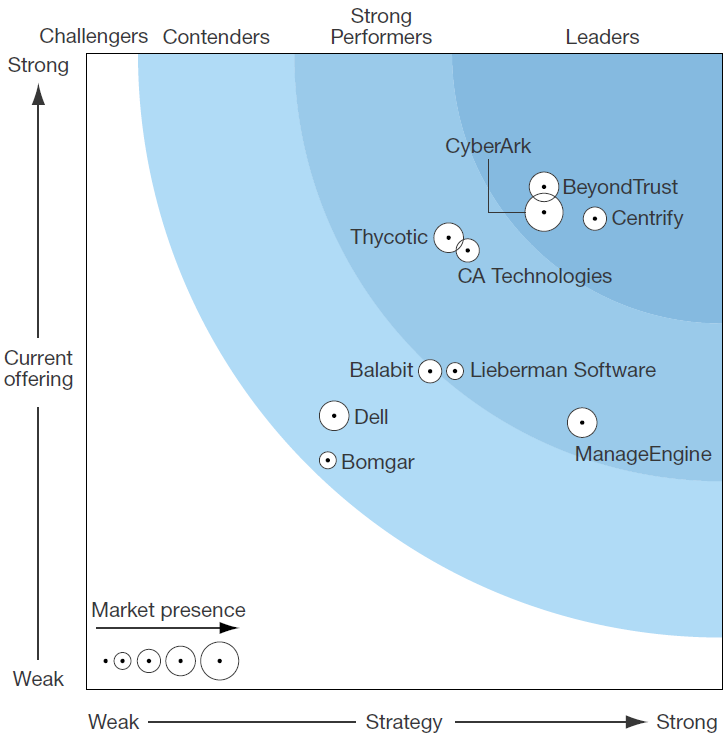
\includegraphics[width=0.7\textwidth]{./images/forrester_quadrant.png}
    \caption{Quadrant mettant en évidence les acteurs du marché de PAM selon le rapport offre/stratégie et l'indice de présence sur le marché}
\end{figure}

Nous avons ainsi pu nous retrouver avec une liste de solutions satisfaisante pour pouvoir commencer à faire un comparatif *réaliste* (terme à revoir). Nous avons alors orienté mes recherches vers les spécificités des solutions, en parcourant toute la documentation disponible, en participant à des vision-conférences avec les commerciaux et ingénieurs des maisons d'édition ou en contactant le support. Cette étape a été celle qui a pris le plus de temps dans la période de recherche, qui parfois s'est avérée infructueuse au vu du manque d'informations disponibles et de l'absence de réponse du support (ou plus précisément des réponses me redirigeant vers des documents en ligne ne contenant pas les réponses demandées).